\documentclass[conference]{IEEEtran}
\IEEEoverridecommandlockouts
% The preceding line is only needed to identify funding in the first footnote. If that is unneeded, please comment it out.
\usepackage{cite}
\usepackage{amsmath,amssymb,amsfonts}

\usepackage{graphicx}
\usepackage{textcomp}
\usepackage{xcolor}
\usepackage{tikz}
\usepackage{verbatim}
\usepackage{algorithm}
\usepackage[noend]{algpseudocode}
\usepackage{multirow}
\usepackage{url}
%\usepackage[sorting=none]{biblatex}
\usepackage[utf8]{inputenc}
\usepackage{ifthen}
\usepackage{filecontents}
\usetikzlibrary{shapes,arrows,shadings,patterns}
\usepackage{pgfplots}
\pgfplotsset{compat=newest}
\pgfplotsset{plot coordinates/math parser=false}

\makeatletter
\def\BState{\State\hskip-\ALG@thistlm}
\makeatother

\usetikzlibrary{positioning}
\def\BibTeX{{\rm B\kern-.05em{\sc i\kern-.025em b}\kern-.08em
    T\kern-.1667em\lower.7ex\hbox{E}\kern-.125emX}}
    
\makeatletter
\def\endthebibliography{%
  \def\@noitemerr{\@latex@warning{Empty `thebibliography' environment}}%
  \endlist
}
\makeatother    
    
\makeatletter
\def\thickhline{%
  \noalign{\ifnum0=`}\fi\hrule \@height \thickarrayrulewidth \futurelet
   \reserved@a\@xthickhline}
\def\@xthickhline{\ifx\reserved@a\thickhline
               \vskip\doublerulesep
               \vskip-\thickarrayrulewidth
             \fi
      \ifnum0=`{\fi}}
\makeatother

\newlength{\thickarrayrulewidth}
\setlength{\thickarrayrulewidth}{3\arrayrulewidth}    
    
\begin{document}

\title{Machine Learning Autoencoder Applied to Communication Channels}


\author{
\IEEEauthorblockN{Eduardo Dadalto Camara Gomes\IEEEauthorrefmark{1}}

%%Meryem Benammar\IEEEauthorrefmark{2}}

\IEEEauthorblockA{\IEEEauthorrefmark{1}Institut Supérieur de l'Aéronautique et de l'Espace (ISAE-SUPAERO), Université de Toulouse, 31055 Toulouse, FRANCE\\
Email: eduardo.dadalto-camara-gomes@student.isae-supaero.fr
}
%\IEEEauthorblockA{\IEEEauthorrefmark{2}Institut Supérieur de l'Aéronautique et de l'Espace (ISAE-SUPAERO), Université de Toulouse, 31055 Toulouse, FRANCE\\
%Email: meryem.benammar@isae-supaero.fr
%}
}

%\IEEEspecialpapernotice{(Final report)}

\maketitle

\begin{abstract}

Communication channel error correction is key to enable digital critical communication systems to work efficiently. The maximum a posteriori (MAP) decoder is proven to be the mathematically optimal solution for the problem. However, its implementation cripples the system applicability. This is because the MAP rule introduces a large delay for long code words. In this context, a deep neural network (DNN) is proposed to optimize the channel with an end-to-end autoencoder. The trained DNN autoencoder has a \textit{one-shot} capability which outperforms a MAP decoder for a given encoder in terms of delay. The decoders proved to be around 25\% faster than the MAP and they achieved the same BER performance. There are still opportunities for enhancement for the autoencoders.

\end{abstract}

\begin{IEEEkeywords}
communication system, machine learning,  autoencoder, channel decoding, maximum a posteriori (MAP) decoder 
\end{IEEEkeywords}

\section{Introduction}
\subsection{Motivation}
A point to point communication channel is a system in which  two terminals exchange information through a noisy channel as Fig. \ref{fig:cs} illustrates. As a result of channel imperfections, Shannon theorized in \cite{Shannon:2001:MTC:584091.584093} the ultimate reliable data rate that can be transmitted through a communication system with an arbitrarily small probability error. 

\begin{figure}[!ht]
  \centering
    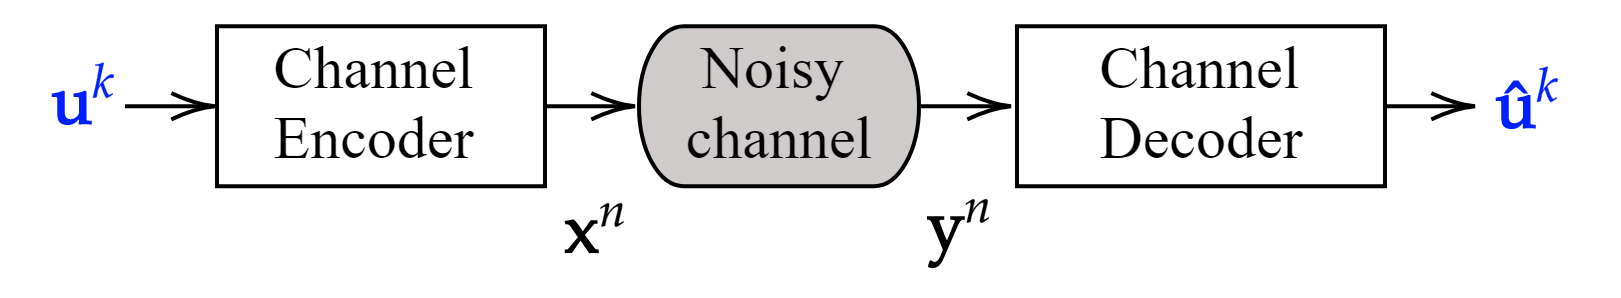
\includegraphics[width=0.5\textwidth]{simple_sys}
    \caption{Diagram of a simplified communication system.}\label{fig:cs}
\end{figure}

Since then, the research community in digital communication developed a series of algorithms to minimize error probability over a channel. In practice, the bit error rate (BER), an approximation of the probability of error, is targeted. However, the challenge of finding an \textit{efficient} solution  i.e., with both low latency and low error probability, for low signal to noise ratio (SNR) channels, remains. Low latency and high bandwidth wireless communication are key to critical systems, such as airplanes, satellites, cellular communication and 5G operations. The latter was studied by F. D. Calabrese et al. in \cite{DBLP:journals/corr/CalabreseWGPS16} which  demonstrated that individual based radio resource management (RRM) algorithms were outperformed by a general learning framework, resulting in significant expense reductions, while increasing performance of the network.

Based on this vision, Tim O'Shea and Jakob Hoydis \cite{DBLP:journals/corr/OSheaH17} pertinently noted that traditional algorithms in the field have foundations in probability theory e.g. maximum a posteriori (MAP) rule, maximum likelihood decoder (MLD) and turbo codes. Hence, they are usually built on top of mathematically convenient models. Even though they are theoretically optimal error corrector codes, these models often do not account for all the real system's imperfections, which leads to errors when implemented in practice.

As opposite to structured algorithms, machine learning (ML) algorithms do not require rigidly designed models and can take non-linearities effortlessly into account. These characteristics make these algorithms candidates for being used as channel decoder. Moreover, with ML based channel encoder and channel decoder, the design of communication systems as independently working blocks becomes obsolete, as a deep neural network (DNN) is able to actuate end-to-end in the system. As a result, an optimized autoencoder with a stochastic layer that models channel's imperfections can substitute the block based representation. Therefore, ML based communication systems could be a better representation of realistic systems and could optimize information transmission of different blocklengths and with low decoding latency, resulting ultimately in gain of bandwidth over standard methods. Thereby, ML algorithms are cardinal for state of the art communication applications. 

\subsection{Related work}

Recently, a significant amount of work in radio communication theory has emerged, introducing ML elements to the communication system. O'Shea et al. in \cite{2016arXiv160806409O} developed a channel autoencoder with optimized impairment and regularization layers to emulate channel impairments. They studied this architecture over an additive white Gaussian noise (AWGN) channel, founding ``some promising initial capacity" for this scheme. In their research, results in terms of BER over SNR for a DNN based autoencoder and for a convolutional neural network (CNN) based autoencoder were treated. They used a range of SNR - from $-10 \text{dB}$ to $15 \text{dB}$ - with QPSK and QAM16 modulation as benchmarks. This analysis was conducted for a binary input message.

    
T. Gruber et. al. in \cite{2017arXiv171008379G} proved that a deep learning-based channel decoder could actually learn a decoding algorithm rather than just being a simple classifier. They introduced code words that were not been used in the training set, and the trained NN was able to correctly decode it. They also observed that structured codes are easier to learn than unstructured ones. NN for structured codes are able to generalize to the full codebook even if they have not seen all the training examples. They trained the NN for very short blocklengths ($N \leq 64$) in order to compare with MAP decoding performance.

\subsection{Problem statement}

In this work, we will implement a ML autoencoder for a  BSC that performs similar to the MAP decoder in real applications for a range of SNR from $-10 \text{dB}$ to $10 \text{dB}$. In its most simple form, a channel autoencoder includes an encoder, a noisy channel and a decoder. Using state-of-the art DNN algorithms to find the best solution of the problem, this work aims to contribute to set up a higher standard in terms of performance in bit-error correction and reduced delay for digital communication applications. In a near future, this disruptive methodology for error correction using ML could replace mathematically optimal decoders which are the current guideline.


\subsection{Notation}
Throughout the work, vectors will be written in bold font weight and may  have a subscript which indicates their layer in a NN and may have a superscript which indicates their size length. In order to homogenize notation, for the encoding phase of the communication system, $\textbf{u}^k$ represents an input \textit{source message} and $\textbf{x}^n$ its correspondent code word. For the decoding portion, $\textbf{y}^n$ represents the output of the noisy channel and $\hat{\textbf{u}}^k$ the estimated source message. These definitions are illustrated in Fig. \ref{fig:cs}.

In addition, every indispensable concept is introduced either in italics or is defined by a commonly used abbreviation present in others scientific works.


\section{Theoretical Background}

\subsection{Channel coding}
Consider the communication system illustrated in Fig. \ref{fig:cs}. The left portion of the chain, the transmitter, wants to communicate a message $\textbf{u}$ through a noisy channel. The right portion of the chain, the receiver, may interpret this possible corrupted stream of bits into the original message. Usually this prediction $\hat{\textbf{u}}$ carry errors which we aim to minimize its probability of occurring. In this scenario, the theory of channel coding discuss possible solutions. 

In particular, linear block codes represented by a pair $(n, k)$ called \textit{code name} will be implemented. Where $k$ is the length of a source message and $n$ is the length of a code word. Briefly, a linear encoder will index a message $\textbf{u}^k \in \mathcal{U} \subseteq \{0,1\}^k$ to a code word $\textbf{x}^n \in \mathcal{X} \subseteq \{0,1\}^n$. This mapping is done by the \textit{generator matrix} $ \textbf{G} $.
\begin{equation}\label{eq:encoding}
\mathbb{E}:\textbf{u} \mapsto \textbf{uG}
\end{equation}

The objective of the receiver is to estimate the original message. The empirical error probability, or a BER, in this process is defined as

\begin{equation}
P_{eb} = \frac{1}{M} \underset{u}{\sum}Pr(\hat{u}\neq u)
\end{equation}
where $M$ is the total amount of bits transmitted, $u$ represents one bit transmitted and $\hat{u}$ its estimation.

The Hamming distance $d_H:\mathcal{X}\mapsto \mathbb{Z}$ is a metric in the word subset which in the context of linear coding is equal to equation \ref{eq:dh}. Noteworthy for the MAP rule, a non zero Hamming distance indicates that there is a block error, and ultimately at least a binary error in the received code word.
\begin{equation}\label{eq:dh}
d_H(\textbf{x},\textbf{y}) = \sum_{i=1}^{n} y_i \text{ XOR } x_i 
\end{equation}  

\subsection{Binary Symmetric Channel}

Briefly, a BSC is a noisy channel with a binary input $X\in \{0,1\}$ on the left and a binary output $Y\in \{0,1\}$ on the right. They are linked through a stochastic model characterized by a crossover probability of value $p$ as illustrated in Fig. \ref{fig:BSC}. Typically, $p$ is smaller than $0.10$.


\begin{figure}[!ht]
  \centering
    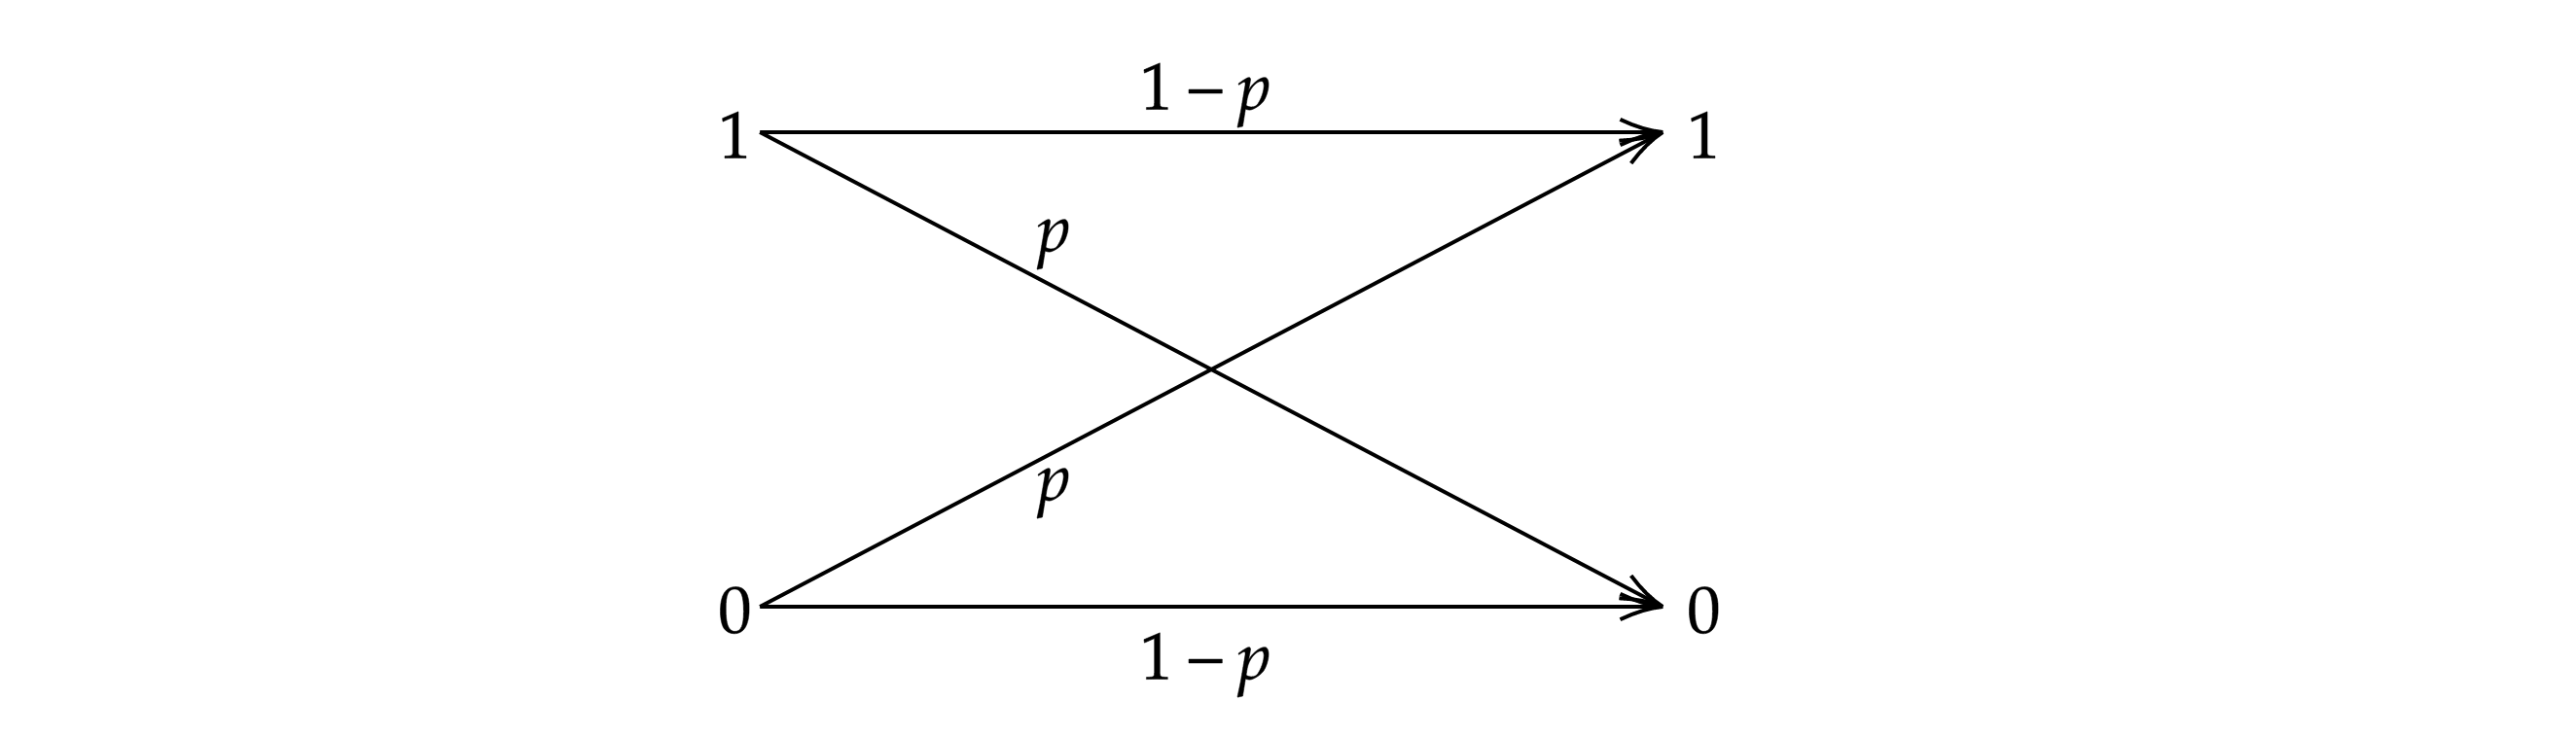
\includegraphics[width=0.4\textwidth]{images/BSC}
    \caption{Illustration of a binary symmetric channel with crossover probability $p$.}\label{fig:BSC}
\end{figure}

A BSC could be represented mathematically through conditional probabilities as follows.

\begin{align*}
Pr[ Y = 0 | X = 0 ] &= 1 - p \\
Pr[ Y = 0 | X = 1 ] &= p \\
Pr[ Y = 1 | X = 0 ] &= p \\
Pr[ Y = 1 | X = 1 ] &= 1 - p
\end{align*}

\subsection{Maximum a posteriori decoder}


The concept of a MAP decoder algorithm for sequences, is choosing a message which maximizes the a posterior probability of the corrupted code word $y$ received by the decoder \cite{Worm00turbo-decodingwithout}. This algorithm is known for its optimal error correction capability for white noise interference. This algorithm is also referred as the Viterbi decoder \cite{Viterbi}.

Mathematically, we want to maximize the average probability of making a correct decision when analysing the channel output $\textbf{y}$, which is written as
\begin{equation}\label{eq:MAP1}
Pc := Pr[\textbf{X}=f({Y})]
\end{equation}
where $x \sim X$ and $y \sim Y$ are multivariate random variables. We derive below the decoder that maximizes $P_c$.

\begin{align} 
\Pr \left[ X=f\left( Y\right) \right]& =\sum_{f\left( y\right) y\in \mathcal{X}\times \mathcal{Y}} P_{XY}(f(y)y) \label{eq:MAP2} \\
&=\sum _{y\in \mathcal{Y}}P_{Y}\left( y\right)P_{X|Y}\left( f(y)|y\right) \label{eq:MAP3}
\end{align}

The optimal decoder is finally given by
\begin{align}
f(y) &= \underset{x\in \mathcal{X}}{\text{arg max}} P_{X|Y}(x|y)\label{eq:MAPF1}\\
&= \underset{x\in \mathcal{X}}{\text{arg max}}
P_X(x)P_{Y|X}(y|x).\label{eq:MAPF2}
\end{align}

However, the MAP decoder is practically nonviable to implement \cite{journals/ett/RobertsonHV97}. Thus, its variants cited in this paragraph are better suited for practical cases. The Log-MAP is an optimal decoder, having equivalent performance to the MAP decoder. While the Max-Log-MAP is a suboptimal decoder and will not be treated in this paper.  these variants are widely used as decoders for turbo codes \cite{HagenauerJ}. Refer to \cite{journals/ett/RobertsonHV97} for specific details in the derivation of the Log-MAP algorithm. Furthermore, the Bahl-Cocke-Jelinek-Raviv (BCJR) algorithm is a bit-wise MAP rule with lower complexity widely used in practice, even for long data packets.

Turbo decoding using Log-MAP decoder for an additive white Gaussian noise (AWGN) channel and for a BSC was studied in \cite{JordanMA}. They analyzed the BER for small SNR and concluded that the results are sensible to SNR estimation of the real channel, since the estimation of this parameter is required for the metric calculation of the algorithm \cite{journals/ett/RobertsonHV97}. It means that if the real SNR is smaller, the decoder will not perform well. Hence, for channel characteristics that change over time, the application of a MAP algorithm is debatable. This conclusion serve as motivation for ML autoencoders, which could adapt to different SNR conditions, outperforming the MAP decoder for realistic applications.

\subsection{Neural network basics}

\tikzset{%
  every neuron/.style={
    circle,
    draw,
    minimum size=0.666cm
  },
  neuron missing/.style={
    draw=none, 
    scale=2,
    text height=0.333cm,
    execute at begin node=\color{black}$\vdots$
  },
}

\begin{figure}[!hbp]
\centering

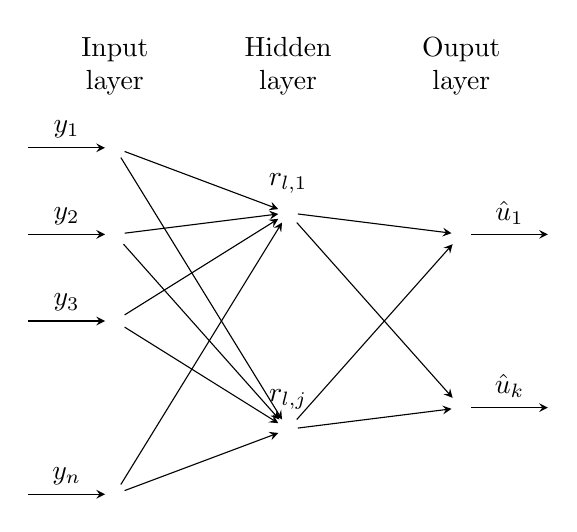
\begin{tikzpicture}[x=1.1cm, y=1.1cm, >=stealth]

\foreach \m/\l [count=\y] in {1,2,3,missing,4}
  \node [every neuron/.try, neuron \m/.try] (input-\m) at (0,2.5-\y) {};

\foreach \m [count=\y] in {1,missing,2}
  \node [every neuron/.try, neuron \m/.try ] (hidden-\m) at (2,2-\y*1.25) {};

\foreach \m [count=\y] in {1,missing,2}
  \node [every neuron/.try, neuron \m/.try ] (output-\m) at (4,1.5-\y) {};

\foreach \l [count=\i] in {1,2,3,n}
  \draw [<-] (input-\i) -- ++(-1,0)
    node [above, midway] {$y_\l$};

\foreach \l [count=\i] in {1,j}
  \node [above] at (hidden-\i.north) {$r_{l,\l}$};

\foreach \l [count=\i] in {1,k}
  \draw [->] (output-\i) -- ++(1,0)
    node [above, midway] {$\hat{u}_\l$};

\foreach \i in {1,...,4}
  \foreach \j in {1,...,2}
    \draw [->] (input-\i) -- (hidden-\j);

\foreach \i in {1,...,2}
  \foreach \j in {1,...,2}
    \draw [->] (hidden-\i) -- (output-\j);

\foreach \l [count=\x from 0] in {Input, Hidden, Ouput}
  \node [align=center, above] at (\x*2,2) {\l \\ layer};

\end{tikzpicture}

\caption{MLNN representative diagram, where $\textbf{y}^n$ is the input vector, $\textbf{r}_{l}^{j}$ is a hidden layer vector
and $\hat{\textbf{u}}^{k}$ is the output vector.} \label{fig:NN}
\end{figure}

Neural networks (NN) are a set of connected \textit{neurons} able to approximate any kind of function through an architecture composed of several single processing units (neurons) connected together forming a network. They are defined by \cite{Ibnkahla} as parallel distributed, learning- and self-organizing information processing systems. 

In the context of learning algorithms implemented by a NN, the key issue is to find a suitable architecture that delivers the best results. To define and build this infrastructure, the activation function, the loss function and the structure must be decided. Nielson \cite{nielsenneural} in his book explores a vast amount of NN architectures and how they work. 

Multi-layer feed forward neural network (MLNN) as shown in Fig. \ref{fig:NN} will be applied in this work. They are known for the universal approximation property \cite{Ibnkahla} and for the versatility of increasing the number of layers, creating a DNN able to undertake complex classification problems with low classification error and low dimensionality. In more general terms, a MLNN with $L$ layers, also called \textit{depth}, and parameter $\theta$ is a mapping of an input $\textbf{y}^n \in \mathbb{R}^{n}$ to an output $\textbf{û}^k \in \mathbb{R}^{k}$ through $L$ iterative steps. For a fully-connected network, each layer vector is calculated iteratively in the forward propagation. Each neuron is composed of a linear combiner and an activation function defined as 

\begin{equation}\label{eq:eqFP}
	f_{l}\left( \textbf{r}_{l-1};\theta _{l}\right) = \sigma \left( \textbf{W}_{l}\textbf{r}_{l-1}+\textbf{b}_{l}\right)
\end{equation}
where $\textbf{W}_{l}\in \mathbb{R} ^{N_{l}\times N_{l-1}}$ is the weight matrix between layers $l-1$ and $l$, $\textbf{r}_{l-1} \in \mathbb{R} ^{N_{l-1}}$ is a vector containing the hidden layer $l-1$ values, $\textbf{b}_{l}\in \mathbb{R} ^{N_l}$ is the bias vector and $\sigma$ is the activation function \cite{DBLP:journals/corr/OSheaH17}.

% TODO: WRITE WHICH ACTIVATION FUNCTION I WILL USE
%
Two common activation functions are the rectified linear unit (ReLU) and the sigmoid function. Both will be applied to the DNNs treated in this paper. In addition, the Softmax activation function is commonly used in multi classification problems and will be used to the One-hot decoding DNN architectures. Their mathematical expressions are shown below.

\begin{align}
	\text{ReLU: } \sigma_1 (x)& = max\{0, x\} \label{eq:relu}\\ 
	\text{Sigmoid: } \sigma_2 (x)& = \frac{1}{1+e^{- \lambda x}} \label{eq:sig}\\
	\text{Softmax: } \sigma_3 (\textbf{z})& = \frac{e^{z_i}}{\sum_{j=1}^{K}e^{z_j}}\label{eq:soft}
\end{align}
where $x \in \mathbb{R}$, $\lambda>0$, $i = 1,...,K$ and $\textbf{z} = (z_1,...,z_K) \in \mathbb{R}^K$.

For a classification problem in communication, the \textit{categorical cross-entropy} loss function $l(\textbf{p},\textbf{q}):\mathbb{R} ^{N_L}\times \mathbb{R} ^{N_L}\mapsto \mathbb{R}$ defined in equation \eqref{eq:c-e} is most common. It is derived from the log-likelihood of a training set where $q_j$ is the estimated probability of the outcome $j$ and $p_{j}$ is the true probability. Basically, the function measures the dissimilarity between $p_{j}$ (what you expected) and $q_{j}$ (what you obtained) \cite{murphy2013machine} where $j=1,...,N_L$. Another commonly used loss function, indispensable for this research, is the \textit{mean squared error} (MSE). The MSE is the  sum of squared distances between our target variable and predicted values and it is defined in equation \ref{eq:mse}. 

\begin{align}
\
	\text{Cross-entropy: }l_1(\textbf{p},\textbf{q}) &=-\sum _{j}p_{j}\log \left( q_{j}\right)\label{eq:c-e} \\
	\text{MSE: } l_2(\textbf{p},\textbf{q}) &=\frac{1}{N_L}\sum _{j}(p_{j}-q_{j})^{2} \label{eq:mse}
\end{align}

With all these elements set, training the neural network to calculate an accurate weight matrix $\textbf{W}$ for forward propagation requires a labeled \textit{training data set}. This set is composed of pairs $ (\textbf{y}_{i}^{n}, {\mathbf{u}}_i^k) $, where $i=1,...,S$ and $S$ is the number of training sets. It matches the input and its respective desired output. The objective is to minimize the overall loss function defined in \eqref{eq:o-c-e} in terms of the parameter $\theta$ \cite{DBLP:journals/corr/OSheaH17}. 
\begin{equation}\label{eq:o-c-e}
L\left( \theta \right) =\dfrac {1}{S}\sum ^{S}_{i=1}l\left({\mathbf{u}}_i^k  , \textbf{y}_{i}^{n}\right)	
\end{equation}  

This problem is an optimization problem and can be solved through different algorithms. For NN, an efficient way of computing this minimization is implementing the back-propagation (BP) algorithm. 	BP is classified as a supervised learning algorithm that is able to optimize a function based on some parameter and is highly parallelizable in computational terms \cite{Ibnkahla}\cite{nielsenneural}.

One of the greatest advantage of NN is its ability to generalize the training set, delivering the right results even for input data not contained in the training set. With the weight matrix trained, the NN finds the correct output values for unseen inputs. In order to validate this principle, a \textit{validation data set} is used and the loss is measured. Based on this value, we can evaluate the NN overall accuracy.

For implementing all the algorithms, Keras, a high-level python API for ML, will be used together with TensorFlow 1.13.1, a ML python friendly open-source library \cite{DBLP:journals/corr/AbadiABBCCCDDDG16} \cite{chollet2015keras}. Both are available on a free license terms.




\subsection{Autoencoders}

Autoencoders based on DNN can learn an appropriate correspondence between input source messages and estimated source message output through different noisy channels. The statistics of the channel's noise is shown in \cite{2017arXiv171008379G} to be irrelevant, since the NN extract it during training phase. The autoencoder applicability is compelling because the weights computed during training can be separated in two groups, one correspondent to the nodes before the channel and one posterior to the channel. As a consequence, we are able to design a non linear encoder and its correspondent non linear decoder with ease. This new representation has ultimately far more possibilities than conventional encoding patterns.

Mathematically, the non linear autoencoder`s encoding function $\phi: \{0,1\}^k \mapsto \{0,1\}^n $ maps the message input to its code word. 

\begin{equation}
x^n = \phi (u^k)
\end{equation} 

Whilst autoencoders are more complex dimensional wise compared to NN decoders, the readily access to graphical processing units (GPUs) contributed to the feasibility of this technique, tackling the \textit{curse of dimensionality} challenge in ML. This type of hardware made possible the approach of the layer-by-layer supervised training by stochastic gradient descent optimization applied in this work. \cite{doi:10.1162/neco.2006.18.7.1527}

A common architecture of DNN autoencoders is shown in Fig. \ref{fig:DDNNAutoencoder} where the encoder and the decoder are composed of dense layers of different widths. In addition, a noise layer and a rounding layer acts on the forward propagation but not on the BP, since their activation functions are not differentiable. More details on the autoencoder's architecture is discussed is section III.  


\begin{figure}[!ht]
  \centering
    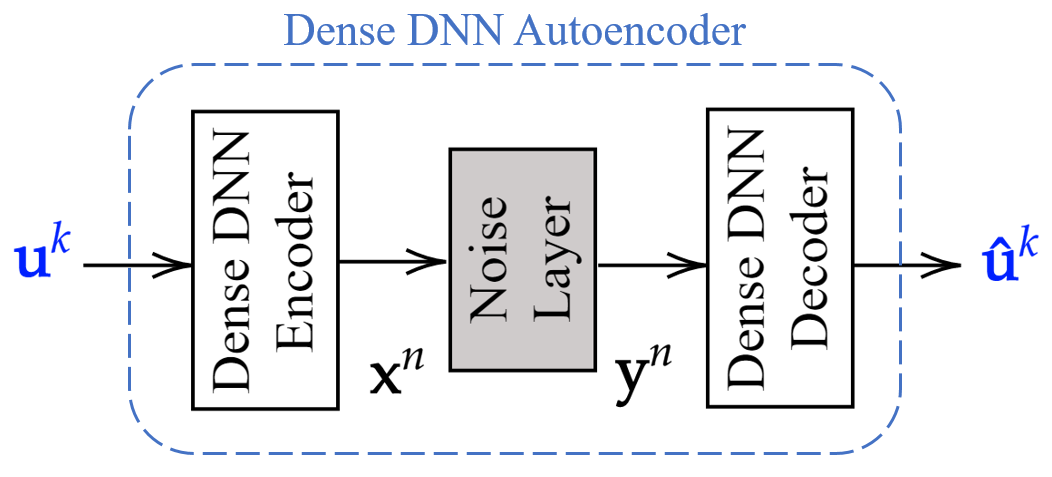
\includegraphics[width=0.4\textwidth]{images/DNN_autoencoder}
    \caption{Representation of a DNN autoencoder composed of dense layers.}\label{fig:DDNNAutoencoder}
\end{figure}



\section{Implementation and Methodology}
This section explains the main implementation procedures in order to replicate the results and understand in depth the methodology behind the work. For organizational purposes, the section is divided into four subsections. First, the predictions and error corrections statistical relevance are justified through the Monte Carlo simulations conducted. Second, the MAP algorithm for a linear code is shown. Then the experiments relating to the ML based decoders are assessed. Finally the implementation of the ML based autoencoder is explained. 

\subsection{Monte Carlo Simulation}

For calculating the BER versus the crossover probability $p$ with confidence over the results, a Monte Carlo simulation was elaborated. This stochastic computational algorithm uses pseudo-random sampling to solve different problems. Hence, we can work with a wide variety of transmission scenarios.

Applied to the context of this research, the messages are repeatedly randomly generated for a specific BSC of crossover probability $p$. They are coded by a linear block code or by a DNN encoder and then transmitted through the channel. Their information arrives corrupted by noise in the decoder and is subsequently partially corrected by a decoder. Finally the average BER is calculated and plotted. The interval of the horizontal axis is in between $0$ and $0.10$.

Every channel is tested with $100000$ messages. As a consequence of the \textit{law of large numbers}, the empirical sampling of the BER represents sufficiently well the real distribution. 

\subsection{MAP Rule}

The MAP algorithm as cited previously, has a high time complexity $(\mathcal{O}(2^k))$, since it computes the Hamming distance between the received code word and every code word from the code book. For more details, the pseudo code of the algorithm is available below.

\begin{algorithm}
\caption{MAP rule for BSC and linear block code.}\label{alg:MAP}
\hspace*{\algorithmicindent} \textbf{Input:} received block $\textbf{y}^n \in \{0,1\}^n$, code word set $\mathcal{X}$ and generator matrix $G_{k \times n}$. \\
\hspace*{\algorithmicindent} \textbf{Output:} message estimation $\hat{\textbf{u}}^k \in \{0,1\}^k$.
\begin{algorithmic}[H]
\Procedure{MAP Decoder}{$y,\mathcal{X}, G$}
\State $\textit{p} \gets \text{channel crossover probability}$
\For{i in \textit{range}($2^k$)}
\State $\text{distances}[i] \gets d_H(\textbf{y},word[i] \in \mathcal{X})$
\EndFor
\State $\hat{\textbf{x}} \gets argmin(\text{distances})$
\State $\hat{\textbf{u}} \gets \hat{\textbf{x}} G^{-1}$
\Return $\hat{\textbf{u}}$
\EndProcedure
\end{algorithmic}
\end{algorithm}

The linear encoding matrix $\textbf{G}_{8\times16}$ was used for the encoding of the messages. Its dimension is equal to the linear block code name represented by the double $(n,k)=(16,8)$. Thus, the \textit{rate} of the code is equal to $0.5$. The linear block name and = rate is constant throughout the work.


\begin{flalign*}
    &\textbf{G}=&
\end{flalign*}

\[
\left [
  \begin{array}{cccccccccccccccc}
  
   1 & 1 & 1 & 1 & 0 & 0 & 0 & 0 & 0 & 0 & 0 & 0 & 0 & 0 & 0 & 0 \\
	1 & 1 & 0 & 0 & 1 & 1 & 0 & 0 & 0 & 0 & 0 & 0 & 0 & 0 & 0 & 0 \\
	1 & 1 & 1 & 1 & 1 & 1 & 1 & 1 & 0 & 0 & 0 & 0 & 0 & 0 & 0 & 0 \\
	1 & 1 & 0 & 0 & 0 & 0 & 0 & 0 & 1 & 1 & 0 & 0 & 0 & 0 & 0 & 0 \\
	1 & 1 & 1 & 1 & 0 & 0 & 0 & 0 & 1 & 1 & 1 & 1 & 0 & 0 & 0 & 0 \\
	1 & 1 & 0 & 0 & 1 & 1 & 0 & 0 & 1 & 1 & 0 & 0 & 1 & 1 & 0 & 0 \\
	1 & 0 & 1 & 0 & 1 & 0 & 1 & 0 & 1 & 0 & 1 & 0 & 1 & 0 & 1 & 0 \\
	1 & 1 & 1 & 1 & 1 & 1 & 1 & 1 & 1 & 1 & 1 & 1 & 1 & 1 & 1 & 1
  \end{array}
\right ]
\]

To establish a reference model to use as comparison base to the DNN models and MAP decoder, the BER results for a scenario without codification was calculated. The ensemble of the no decoding curve and the MAP algorithm curve of Fig. \ref{fig:MAP} are replicated for comparison purposes with the methods of interest.

\begin{figure}[!ht]
  \centering
    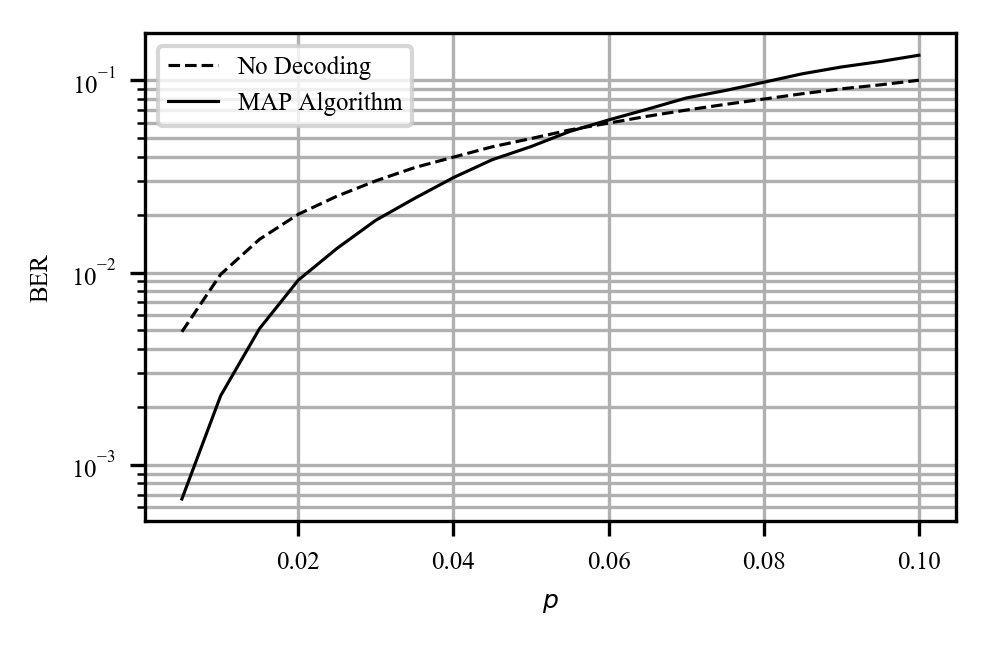
\includegraphics[width=0.5\textwidth]{images/MAP-alone-curve}
    \caption{No decoding and MAP algorithm performance in terms of BER versus channel crossover probability.}\label{fig:MAP}
\end{figure}

\subsection{Decoder}

This section is divided in two for better identify the differences between the implementation of the array DNN decoder and the one-hot DNN decoder.

\subsubsection{Array Decoder}

The architecture of the DNN necessary to achieve a great performance in terms of BER is not evident. To begin we must define which layers were used and why. A \textit{Lambda} layer is a layer in which the activation function is user defined and the parameters are non-trainable. Thus, we were able to define a layer that act as a BSC to force our DNN to learn its effects in the training data. The fact that the parameters are non-trainable means that the noise layer is applied in forward propagation only. A Dense layer is a densely connected layer, which means that each neuron receives input from all the neurons in the previous layer. Thus it is often used to change the dimensions of a vector. In other words, it applies a rotation, scaling and translation transform to a vector as shown in equation \ref{eq:eqFP}. The values in the weight matrix are trainable parameters which are updated during BP \cite{chollet2015keras}.

The choice of the crossover probability of the training channel, $p_{t}$, was based in the work of \cite{DBLP:conf/acssc/BenammarP18} which shows $p_{t}=0.07$ to be the best in terms of decoding precision after the DNN is trained. In addition, a deeper DNN showed best results in \cite{DBLP:journals/corr/OSheaH17} where 3 hidden layers were used. Consequently, the same architecture were adopted to solve the problem as shown in table \ref{tab:arraydecoder}. 

\begin{table}
\caption{DNN array decoder architecture.} 
\begin{center}

  \begin{tabular}{ l  |  l }
    \thickhline
    Channel &  Lambda: $\textbf{x}\oplus \text{noise}$\\ \hline
    \multirow{3}{*}{Decoder} & Dense: 128, activation: ReLU, input size: 16 \\
 & Dense: 64, activation: ReLU  \\
 & Dense: 32, activation: ReLU  \\
 & Dense: 8, activation: Sigmoid  \\ \hline
    \multicolumn{2}{l}{\textbf{Total parameters: $12776$}}\\
    \thickhline
  \end{tabular}
    \label{tab:arraydecoder}
\end{center}
\end{table}

\begin{table}
\caption{DNN array decoder training parameters.} 
\begin{center}
\begin{tabular}{ l  |  l | l | l  }
    \thickhline
 Loss func. & Optimizer & N. Epochs & Batch Size \\ \hline
 Binary cross-entropy & Adam & $2^{16}$ & $256$ \\
    \thickhline
  \end{tabular}
    \label{tab:arraydecoderTrain}
\end{center}
\end{table}

The training set for the array decoder contained all the possible messages as training labels and its correspondents code words as training data. Because of the chosen encoding, the training data is a $256\times16$ matrix and the training label is a $256\times8$ matrix. To generate a possible message, a stochastic algorithm was developed to fabricate random 8-length vectors of integers 1s and 0s which the average value considering all elements was around $0.5$. In this way we could guarantee that our training environment were representative of a real life application. Where different bits are transmitted with the same probability.

Even though it is not recommended to train a NN with all the available data - because it might lead to over-fitting -, for this case does not seems to be a problem. WHY????? (noisy channel? onehot decodeR?)

The choices of training parameters is a mix between what other works in literature uses and a hyper parametric analytic approach, where several trials lead to the decision. First, the binary cross-entropy as loss function is widely used in literature and  showed to converge to the desired result consistently during tests. For the optimizer, the \textit{Adam} built-in Keras optimizer was chosen. Adam optimizer algorithm is similar to a classic stochastic gradient descent algorithm, but computes individual adaptive learning rates for different parameters from estimates of first and second moments of the gradients \cite{chollet2015keras}. Next, a batch size matching the size of the training set which is sufficiently small to still operate in the regime of small batch was chosen. In \cite{DBLP:journals/corr/KeskarMNST16}, the authors demonstrated better performance for a NN training with stochastic gradient descent and its variants operating in a small-batch regime, usually between 32-512 data points. Finally, the necessary number of epochs to training is sensitive to the problem, since it impacts directly the training computational cost. As a result, we tried several training epoch sizes and found $2^{16}$ to have precise results and be computationally viable. The training parameters are displayed in table \ref{tab:arraydecoderTrain}.


\subsubsection{One-hot Decoder}

The architecture of the one-hot decoder is much simpler when compared to the array decoder. It contains only one layer of $256$ units which maps the input of size 16 to the $2^8=256$ possible messages. Hence, this characterizes a multi-class classification problem, meaning that the chosen activation function is the Softmax (Eq. \ref{eq:soft}). This training technique is known in the literature as \textit{one-hot}. 

The denomination one-hot comes from the output vector which is usually a long vector of zeros with one element equals to one. This \textit{hot} vector element indicates which class the NN has classified the input. In this context, which message encoded in 256 different classes the code word refers to. Basically, a message is mapped into a class and a class only.

A straight forward consequence of this shallower NN is the number of training parameters almost three times less than the array decoder. Because of that, we could expect a lower training time. Also, we observed that the number of training epochs is substantially smaller for the one-hot decoder. It was necessary only $2^{14}$ epochs to achieve the results for the same batch size of $256$ and Adam optimizer.

Despite the NN complexity benefits of the one-hot decoder, it is required to transform the predicted vector into a message. Consequently, an additional operation is needed. To transform from a one-hot vector to a message, a ordered collection of the messages was stored in memory and the correspondent message is determined by a $argmax$ operation in the one-hot vector, which identifies which message is the most likely to have been transmitted through the channel.

The training set in this case differs from the array decoder. The training labels are one-hot vectors which maps into real messages through a bijective function. Thus, it is a matrix of dimension $256\times256$ composed of 256 different on-hot vectors. The training data is still the linear encoding of the real messages by the matrix $\textbf{G}$. 

The one-hot decoder was trained both with and without a noise layer. The model without a integrated channel converged faster to the solution. Tables \ref{tab:onehotdecoder} and \ref{tab:onehotdecoderTrain} resume the architecture and training variables, respectively.

\begin{table}
\caption{DNN one-hot decoder architecture.} 
\begin{center}

  \begin{tabular}{ l  |  l }
    \thickhline
    \multirow{1}{*}{Decoder} & Dense: 256, activation: Softmax, input size: 16 \\ \hline
    \multicolumn{2}{l}{\textbf{Total parameters: }$4352$}\\
    \thickhline
  \end{tabular}
    \label{tab:onehotdecoder}
\end{center}
\end{table}

\begin{table}
\caption{DNN one-hot decoder training parameters.} 
\begin{center}
\begin{tabular}{ l  |  l | l | l  }
    \thickhline
 Loss func. & Optimizer & N. Epochs & Batch Size \\ \hline
 Binary cross-entropy & Adam & $2^{14}$ & $256$ \\
    \thickhline
  \end{tabular}
    \label{tab:onehotdecoderTrain}
\end{center}
\end{table}

Even though DNN encoders are useful, an encoding matrix is still needed. With a view to eliminate completely the need of an explicit encoding, a technique commonly used method in ML for image recognition is explored. The autoencoder is able to learn not only a decoding algorithm, but also a decoding one as introduced in the following section.

\subsection{Autoencoder}
For the DNN autoencoder, two different concepts were studied. The array autoencoder takes as input the messages and it tries to replicate them, encoding it in a 16 bit code word, transmitting through a noisy channel and decoding it in the second portion of the NN. A one-hot autoencoder is inputted by a one-hot vector representing one unique k-bit message. It encodes the vector into a n-bit long code word, transmits it through a noisy channel and decode it in the second part of the NN. 

This end-to-end approach for both architectures is promising for digital communication, since there is no need for a predefined linear encoding. Theoretically, the DNN could learn the best encoding and associated decoding to a specific channel. Once trained, they could perform optimally in terms of encoding and decoding for a channel. To be clear during the discussion of this and the following sessions, the autoencoder will be divided in: the encoder, the channel and the decoder portions as shown in Fig. \ref{fig:DDNNAutoencoder}. In total, there were tested 71 array and 80 one-hot autoencoders different architecture or training configuration.

\subsubsection{Array Autoencoder}

Even though in theory the autoencoder could be able to achieve at least the same MAP performance, finding the parameters which unveils its capabilities requires multiple testing and a rigorous hyper-parametric analysis. For the array autoencoder, we first experimented with the depth of the encoder. The number of hidden layers in a DNN has influence in the BP algorithm. Extremely deep NN, with more than 4 hidden layers, may encounter problems in the gradient calculations due to vanishing weights. When the weights becomes too small, they may be source of underflow, depending on the machine precision. 

The encoder portion was first analyzed in a standalone session. We trained the encoder to replicate the linear encoding proposed in the preceding sections as we studied the effects of each parameter in the training performance. A more wide architecture showed faster convergence and the use of three hidden layers had no positive effects. In the end, for the integrated model we opted for using two hidden layers, with 512 and 256 densely connected units as detailed in table \ref{tab:arrayautoencoder}. The activation functions remained the same as in the DNN decoders discussed in the previous section.

Integrating the channel in the autoencoder model posed a challenge.  The prediction of the encoder outputs a real vector with elements in the codomain $(0,1)$ of the sigmoid function. Henceforth, a rounding function is mandatory for the channel transmission. The issue is that a rounding function is not differentiable in zero. This would stop the BP as no gradient would be computed. The solution was to only round values in the forward propagation and ignore this function during BP. The command \textit{tf.keras.backend.stop\textunderscore gradient} in a python environment with \textit{tf.keras} as backend does exactly what we wanted and was implemented in the rounding lambda layer. 

The decoder architecture was also based on the standalone array decoder. In spite of this, there were no difference outstanding in decoding with or without the last hidden layer of the decoder. In the other hand, the tests with a condensate NN with one hidden layer demanded a greater training time to arrive in the same results. The final test was done with the entire autoencoder and the final tweaks were done.

While training the autoencoder we noticed that the binary cross-entropy loss function would need more training epochs than the MSE and \textit{logcosh} loss functions, even though they converged in similar results. The batch size was maintained as the size of the first dimension of the training set and there was no reason for changing the optimizer. Notwithstanding, the ensemble of changes and optimizations were not enough to find a suitable architecture for channels with $p<0.02$ as the MAP algorithm for the 1/2 rate encoder would do better in this scenario. Table \ref{tab:arrayautoencoderTrain} summarizes the array autoencoder training parameters.

Furthermore, adding batch normalization layers inside the DNN was fundamental. With greater training parameters, achieving convergence in a reasonable time requires more computing power without any specific technique. The constant changes of weight values in the intermediate layers in every training step is the principal contributor to training cost. This problem is known as \textit{internal covariance shift}. What batch normalization does is normalize the input of a layer by its batch statistics and then scale and shift it. For further details, refer to \cite{DBLP:journals/corr/IoffeS15}.

The final parameter to determine is the training channel cross over probability. Once the architecture and training parameters were defined, a simulation for the same DNN with different $p_t$ was done and the trained models were analyzed in terms of BER. A $p_t=0.03$ yielded best performance.


\begin{table}
\caption{DNN array autoencoder architecture.} 
\begin{center}

  \begin{tabular}{ l  |  l }
    \thickhline
    \multirow{3}{*}{Encoder} & Dense: 512, activation: ReLU, input size: 8 \\
   &  Batch normalization \\
 & Dense: 256, activation: ReLU \\
 &  Batch normalization \\
 & Dense: 16, activation: Sigmoid  \\ \hline
 
    \multirow{2}{*}{Channel} & Lambda: $Round(\textbf{x})$, input size: $16$ \\
 & Lambda: $\textbf{x}\oplus \text{noise}$\\ \hline
 
 \multirow{2}{*}{Decoder} & Dense: 128, input size: 16 \\
 &  Batch normalization \\
 & Dense: 64, activation: ReLU  \\
 &  Batch normalization \\
 & Dense: 8, activation: Sigmoid  \\ \hline
 
    \multicolumn{2}{l}{\textbf{Total parameters: }154072}\\
    \thickhline
  \end{tabular}
    \label{tab:arrayautoencoder}
\end{center}
\end{table}

\begin{table}
\caption{DNN array autodecoder training parameters.} 
\begin{center}
\begin{tabular}{ l  |  l | l | l  }
    \thickhline
 Loss func. & Optimizer & N. Epochs & Batch Size \\ \hline
 MSE & Adam & $2^{17}$ & $256$ \\
    \thickhline
  \end{tabular}
    \label{tab:arrayautoencoderTrain}
\end{center}
\end{table}

\subsubsection{One-hot Autoencoder}

The procedure to implement the one-hot autoencoder was similar to the array's autoencoder one. Briefly, it was shown experimentally that for this model, a deeper encoder with layers of gradually decreasing number of units were more suited. We tried both a wider and shallower architecture and a deeper and narrow architecture. The second had better BER performance. The final architecture is available in table \ref{tab:onehotautoencoder}.

In terms of noise, their presence in the channel degraded vastly the results, as the DNN was not able to learn. The challenge of the one-hot encoder implementation is the fact that we are trying to represent a 256 size length vector into a 16 length vector to transmit through the specified channel. The hypothesis is that it requires several steps to converge into a representative state. Thus, no noise channel was implemented, only a rounding layer.

The decoder utilized has fewer layers than the array autoencoder, however more parameters. In terms of activation functions, there is no difference from the DNN one-hot decoder, which utilized a multi-class classification framework as well. In addition, batch normalization proved to be valuable and accelerated the overall training of the DNN.

Apart from the number of training epochs, the other training parameters are identical to the array autoencoder. As table \ref{tab:onehotautoencoderTrain} shows, the one-hot autoencoder utilized two times less training epochs to converge.

\begin{table}
\caption{DNN one-hot autoencoder architecture.} 
\begin{center}

  \begin{tabular}{ l  |  l }
    \thickhline
    \multirow{3}{*}{Encoder} & Dense: 196, activation: ReLU, input size: 256\\
   & Batch normalization \\
 & Dense: 128, activation: ReLU  \\
 & Batch normalization \\
 & Dense: 96, activation: ReLU  \\
 & Batch normalization \\
 & Dense: 64, activation: ReLU  \\
 & Batch normalization \\
 & Dense: 32, activation: ReLU  \\
 & Batch normalization \\
 & Dense: 16, activation: Sigmoid  \\ \hline
 
   Channel & Lambda: $Round(\textbf{x})$, input size: $16$ \\ \hline
 
 Decoder & Dense: 128, activation: ReLU, input size: 16 \\
 & Batch normalization \\
 & Dense: 256, activation: Softmax  \\ \hline
 
    \multicolumn{2}{l}{\textbf{Total parameters: }134052}\\
    \thickhline
  \end{tabular}
    \label{tab:onehotautoencoder}
\end{center}
\end{table}

\begin{table}
\caption{DNN one-hot autodecoder training parameters.} 
\begin{center}
\begin{tabular}{ l  |  l | l | l  }
    \thickhline
 Loss func. & Optimizer & N. Epochs & Batch Size \\ \hline
 MSE & Adam & $2^{16}$ & $256$ \\
    \thickhline
  \end{tabular}
    \label{tab:onehotautoencoderTrain}
\end{center}
\end{table}


\section{Results and Analysis}

This section is divided in three parts. The first shows the results obtained to the two decoders. Secondly, the results for the autoencoders is brought with some observations during the training period. The discussion and analysis for these two subsections is around the BER performance. Finally, a decoding time performance analysis is done and the results are shown and discussed.

\subsection{Decoders}

We can infer from figures \ref{fig:ArrayD} and \ref{fig:1HD} that both the array decoder and the one-hot decoder are able to learn a decodification function. Moreover,  its performances replicate the MAP algorithm's decoding capability for this specific encoding. Hence, DNN decoders could substitute the mathematically optimal MAP decoder for a stochastic channel, without compromising the bit error probability.

\begin{figure}[!ht]
  \centering
    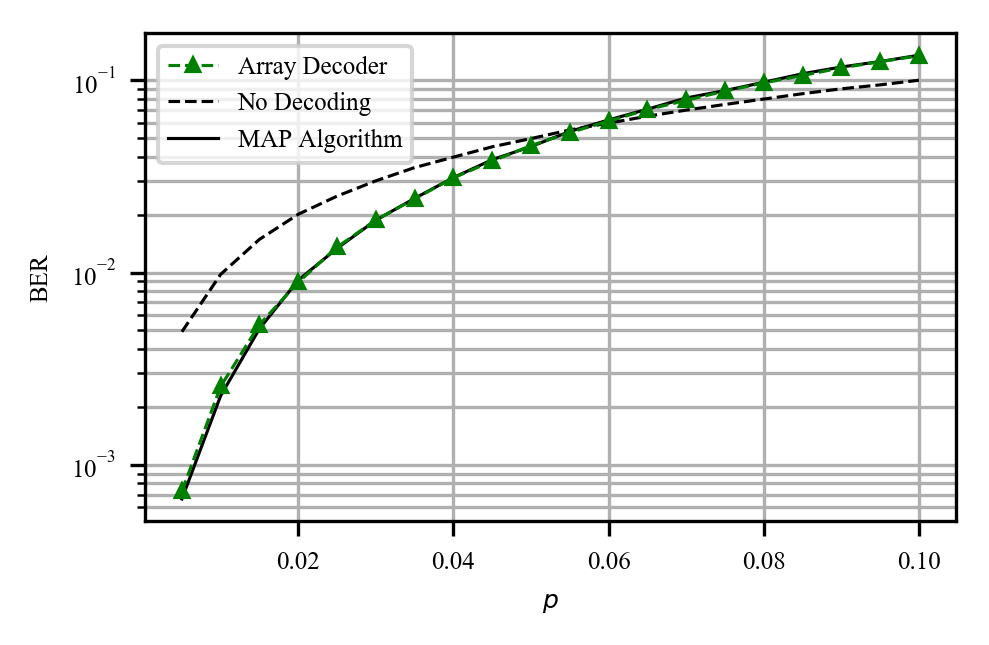
\includegraphics[width=0.5\textwidth]{images/MLNN_Mep_65536_ptrain_007}
    \caption{Array decoding BER performance. DNN array decoder trained with a channel crossover probability error of $p_t=0.07$.}\label{fig:ArrayD}
\end{figure}

\begin{figure}[!ht]
  \centering
    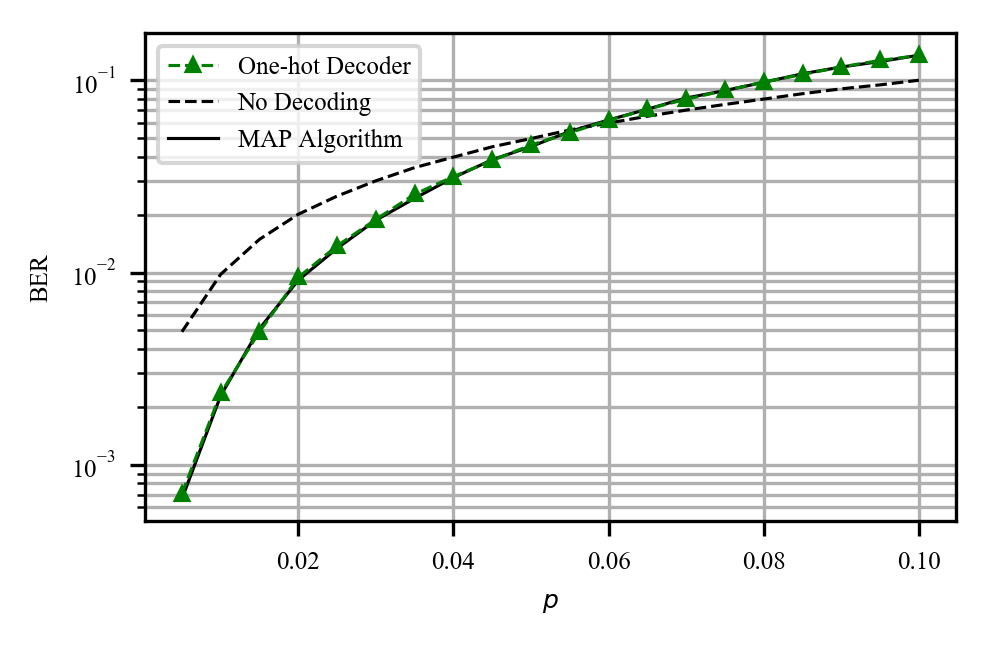
\includegraphics[width=0.5\textwidth]{images/MLNN1H_Mep_16384_ptrain_0}
    \caption{One hot decoding BER performance. DNN one-hot decoder trained without a noisy channel.}\label{fig:1HD}
\end{figure}

The MAP decoder and the DNN decoders were tested with the same number of messages and channels. As a result, since they express the same results, we can assume that the DNN decoder was able to learn the MAP algorithm during training phase. More interestingly, is the convergence period for each decoder. The one-hot decoder reached its peak performance much faster in comparison with the array decoder in terms of training epochs. I would attribute this increased performance to the activation function of the last layer. The sigmoid function used in the array decoder may lead to sharp damp gradients, gradient saturation or slow convergence during BP. While the one-hot decoder uses the softmax function which its partial derivatives have a better behavior during BP. Refer to \cite{2018arXiv181103378N} for deeper details in each activation function characteristics.


\subsection{Autoencoders}
BER Curves of simulation varying p, best choice of p, analyse autoencoder with best choice of p

In the beginning we expected that the autoencoders would beat the MAP algorithm performance for a fixed linear block encoding. They were supposed to learn a non linear encoding and its particular MAP rule which would perform better than the studied MAP for a low crossover probability range. It turned out, however, since there are an enormous amount of possible non-linear codes, it is difficult to the learning algorithm to find the best one. Often during training, the DNN would find a local minimum which its cost function would be very close to zero, even though its performance during prediction phase was far from optimal.

We observed during training, while experimenting with different architecture, that the array autoencoders would have a BER performance which looked like the no decoding curve, but translated in the $y$ axis. This phenomenon can be observed in figure \ref{fig:parrayanalysis} where we tested several $p_t$ options to find the best one for implementing a more refined training. It is remarkable how the curves tend to replicate the same type of behavior. I believe it shows how the local minimums of the solution space of a NN are indeed close to each other, and the weight values may not be indeed that different.

\begin{figure}[!ht]
  \centering
    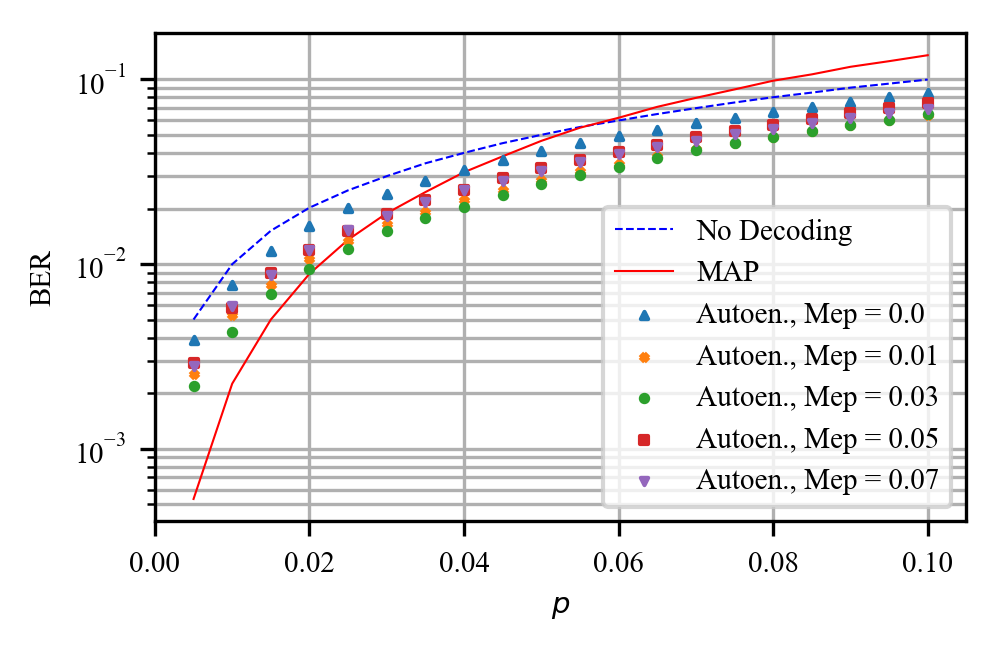
\includegraphics[width=0.5\textwidth]{images/MAP_AutoencoderArray_Mep_65536_64_128_256_p_analysis}
    \caption{Training crossover probability simulation for the array autoencoder. $P_t=0.03$ demonstrated to have best performance to this particular architecture. The DNNs were trained with $2^{16}$ training epochs.}\label{fig:parrayanalysis}
\end{figure}


\begin{figure}[!ht]
  \centering
    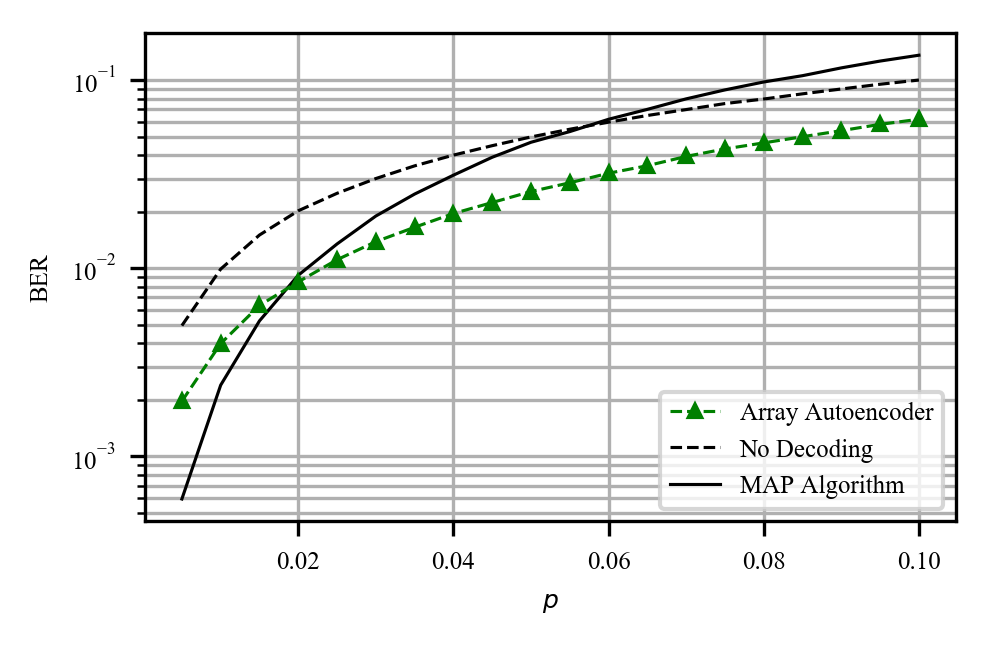
\includegraphics[width=0.5\textwidth]{images/AutoencoderArray_Mep_65536_ptrain_003_logcosh}
    \caption{Array autoencoder BER performance. DNN array autoencoder trained with a channel crossover probability error of $p_t=0.03$. The DNN was trained with $2^{17}$ training epochs.}\label{fig:arrayautoencoder}
\end{figure}

However, it is noticeable the difference in error decoding in terms of a DNN trained with a $p_t=0$ and $p_t=0.3$ in Fig. \ref{fig:parrayanalysis}. Just similar to the array decoder, introducing a channel noise of some kind is beneficial to having a better error correction capability. Using noise also helps in the regularization of the DNN and approximates the training to the real application. 

We can observe from Fig. \ref{fig:arrayautoencoder} that for $p<0.02$, the autoencoder performance is actually worse than the tested MAP algorithm. Several hypothesis were considered for this comportment. In order to test them, we calculated the MAP rule for the encoder learned by the array autoencoder. The error correction yielded the same results as the DNN decoder learned by the autoencoder. Thus, the decoder replicates well the MAP for this specific encoding. Then, we experimented with training parameters and architecture, but could not find a configuration which would perform better than the traced MAP for low values of $p$.


The one-hot autoencoder could not outperform the MAP traced for any value of $p$. As observed in Fig. \ref{fig:1Hautoencoder}, even though it learned a similar encoding, the resulting BER estimation is not optimal. Equally to the array autoencoder, we tested a MAP rule for the learned encoder and found that the DNN decoder portion performs just like the MAP. Thus, once again the problem is in the learned encoding. We tried 80 different configurations, though we could not find one which could outperform the reference model. We can also highlight the trace of the BER curve, approximating the reference model one. Other one-hot autoencoders showed similar curves but translated up in the $y$ axis.



\begin{figure}[!ht]
  \centering
    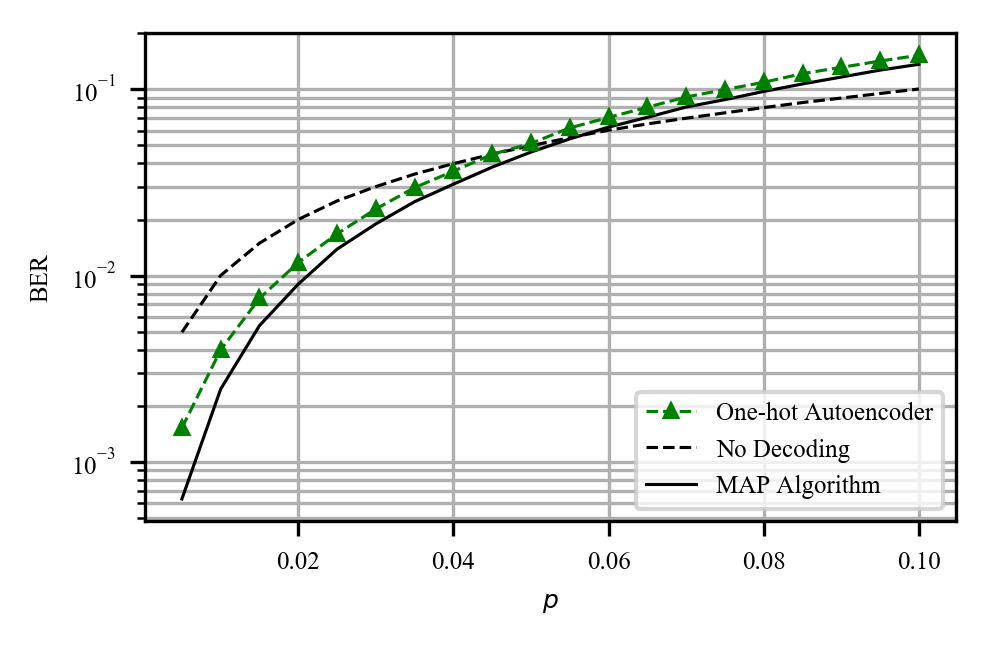
\includegraphics[width=0.5\textwidth]{images/MAP_Autoencoder1H_Mep_131072_ptrain_0_192_128_96_64_32-128}
    \caption{One-hot autoencdoer BER performance. Trained without a noisy channel. The DNN was trained with $2^{16}$ training epochs.}\label{fig:1Hautoencoder}
\end{figure}

\subsection{Decoding time analysis}

In order to analyze the delay in the communication for each technique studied, a Monte Carlo simulation was conducted. There were selected 20 different BSC channels. For each channel, $100000$ messages were codified, transmitted and decodified for each decoder, autoencoder and MAP. This process was timed and repeated several times. In the end, an average time and standard deviation of the results were recorded. A normalization for the average MAP decoding time was done. The results are available in the table \ref{tab:timeanalysis}.  

Both decoders using the linear encoding performed around 25\% faster than the MAP rule. This is due their fairly low dimensional complexity and one shot feature. While the MAP rule must calculate the distance between the received codeword to every possible codeword, the decoders once trained are able to decode the received code word into the message of highest probability with simple matrix multiplications. The latter efficiency is potentialized when using decoding computers equipped with GPUs.

In spite of the one-hot decoder has considerably fewer parameters than the array decoder, it must calculate a $argmax$ function to deliver the actual message that was transmitted. This extra costly computation is also the reason for the increased time for the one-hot autoencoder. It must first encode the message, then transmit it and finally decode it, performing two times per message a $argmax$ operation.

\begin{table}
\caption{Decoding time comparison between the MAP algorithm and the DNN decoders and autoencoders. The data is normalized to the average MAP algorithm decoding time. The simulation was based on CPU calculations. } 
\begin{center}

  \begin{tabular}{ c | c | c}
    \thickhline
    MAP & Array Decoder & One-hot Decoder\\
    $1.00 \pm 0.02$ & $0.74 \pm 0.03$ & $0.76 \pm 0.02$ \\ \hline
    \multicolumn{2}{c|}{Array Autoencoder}  & One-hot Autoencoder\\
   
     \multicolumn{2}{c|}{$1.33 \pm 0.05 $} & $3.02 \pm 0.06$ \\ 
    \thickhline
  \end{tabular}
    \label{tab:timeanalysis}
\end{center}
\end{table}

paragraph that talks about CPU, not GPU.

\section{Conclusions}

The feasibility of a machine learning based channel decoder and the end-to-end application of a deep neural network autoencoder were demonstrated for a communication system with a binary symmetric channel. Their performances were assessed and analyzed in terms of bit error rate performance and communication delay. A few hyper-parametric analysis were conducted to find the best solution for each technique.

The designed decoders improved around 25\% the channel delay when compared to the maximum a posteriori rule for a $(n,k)$ code with $\textbf{G}$ aforementioned as linear encoding matrix. Their small number of parameters aligned with a GPU equipped decoding computer is promissory to be a substitute of the MAP rule and achieve same bit error correction rate. In addition, their training and architecture are straightforward and can be trained with a commercial computer. Once trained, they work as a non-linear decoder to a specific channel encoding.

We also proved that autoencoders can learn a non linear encoding function and its decoding function for a binary symmetric channel. Thus there is no need for a generator matrix for error correction. There are still some challenges in training to solve, such as ameliorate the architecture so it can outperform the reference model in every channel condition. In addition, because of the number of parameters, their calculation in CPU is slow and they showed a greater delay when compared to the MAP rule. Though, they must take the most advantage of GPU based calculations and the delay time could be improved using this technology.

A more rigorous hyper-parametric analysis could find a combination of parameters which yields better BER performance for the autoencoders and is strongly suggested for future work. In addition, in the future, a real implementation of the DNN decoders could be tested to confirm their capabilities as it is not the main focus of this work. We suggest using more advanced NN topology such as a recurrent neural network (RNN) or a generative adversarial network (GAN). Their implementation and training are more complex, however they have recently demonstrated outstanding results in other fields.


%Talk about feasibility of decoders, improved performance of the channel delay with DNN decoders, challenges in implementing this architecture in real life, challenges in training the NNs, Future work, what else could be done with NN in error correction, Advantages and disadvantages in comparison with linear decoding.

\section*{Acknowledgment}

I would like to thank the guidance and advice from my supervisor Meryem Benammar, Ph.D, my colleague Rémy Zawislak who worked in the same theme and collaborated indirectly to the research and Marjorie Grzeskowiak Lucas, Ph.D, who through the Institut Supérieur de l'Aéronautique et de l'Espace (ISAE-SUPAERO) enabled the confection of the project.


%\cite{Shannon:2001:MTC:584091.584093, DBLP:journals/corr/CalabreseWGPS16, DBLP:journals/corr/OSheaH17, 2016arXiv160806409O, 2017arXiv171008379G, Worm00turbo-decodingwithout, Viterbi, journals/ett/RobertsonHV97, HagenauerJ, JordanMA,Ibnkahla, nielsenneural, murphy2013machine, DBLP:journals/corr/AbadiABBCCCDDDG16, chollet2015keras, doi:10.1162/neco.2006.18.7.1527, DBLP:conf/acssc/BenammarP18, DBLP:journals/corr/KeskarMNST16, DBLP:journals/corr/IoffeS15,2018arXiv181103378N}

\bibliographystyle{ieeetr}
\bibliography{bib/ShannonCE1948,bib/CalabreseWGPS16,bib/OSheaH17,bib/Oshea2,bib/Gruber,bib/Worm,bib/Viterbi,bib/RobertsonHV97,bib/HagenauerJ,bib/JordanMA,bib/Ibnkahla,bib/Nielsen,bib/Murphy,bib/AbadiABBCCCDDDG16,bib/Keras,bib/mit_neco18_1527,bib/BenammarP18,bib/KeskarMNST16,bib/IoffeS15,bib/ActivationF}

%\bibitem{b1} C. E. Shannon, ``A mathematical theory of communication," Bell System Technical Journal, vol. 27, no. 3, pp. 379–423, Jul. 1948.


%\bibitem{b3} F. D. Calabrese, L. Wang, E. Ghadimi, G. Peters, and P. Soldati, ``Learning radio resource management in 5G networks: Framework, opportunities and challenges," arXiv preprint arXiv:1611.10253, 2016.

%\bibitem{b2} O'Shea, Tim \& Hoydis, Jakob, ``An Introduction to Machine Learning Communications Systems", 2017.

%\bibitem{osheaautoencoder} T. O'Shea, K. arra, T. C. Clancy, ``Learning to Communicate: Channel Auto-encoders, Domain Specific Regularizers, and Attention", 2016.

%\bibitem{2018} T. Gruber, S. Cammerer, J. Hoydis, and S. ten Brink, “On deep learning based channel decoding,” accepted for CISS 2017, arXiv preprint arXiv:1701.07738, 2017.

%\bibitem{b4} W. Alexander, H. Peter \& W. Norbert, ``Turbo-Decoding Without SNR Estimation",IEEE Communications Letter, vol. 4, no. 6, pp. 193-195, 2000.

%\bibitem{viterbi} A. J. Viterbi, ``Error Bounds for Convolutional Codes and an Asymptotically Optimum Decoding Algorithm", IEEE Transactions on Information Theory, 13 (2): 260–269, 1967.

%\bibitem{b6} Robertson, P. , Hoeher, P. and Villebrun, E. (1997), Optimal and sub‐optimal maximum a posteriori algorithms suitable for turbo decoding. Eur. Trans. Telecomm., 8: 119-125. doi:10.1002/ett.4460080202.

%\bibitem{b7} J. Hagenauer,P. Robertson, L. Papke: iterative (“Turbo”) decoding of systematic convolutional codes with the MAP and SOVA algorithms. In: ITG-Fachbericht 130. October 1994, p. 21-29.

%\bibitem{b5} M. Jordan and R. Nichols, “The effects of channel characteristics on turbo code performance,” in Proc. Milcom’96, McLean, VA, Oct. 1996, pp. 17–21.

%\bibitem{b9} I. Mohamed, ``Applications of neural networks to digital communications - a survey", 1997.

%\bibitem{b8} M. Nielsen, \textit{Neural Networks and Deep Learning}.

%%\bibitem{b10} M. Kevin, ``Machine Learning: A Probabilistic Perspective", MIT, ISBN 978-0262018029, 2012.

%\bibitem{b11} M. Abadi, A. Agarwal, P. Barham, et al.,``TensorFlow: Large-scale machine learning on heterogeneous systems", 2015. Software available from tensorflow.org.

%\bibitem{b12} F. Chollet, “keras,” https://github.com/fchollet/keras, 2015.

%\bibitem{GPU} G. E. Hinton, S. Osindero, and Y.-W. Teh, “A fast learning algorithm for deep belief nets,” Neural Computation, vol. 18, no. 7, pp. 1527–1554, July 2006.

%\bibitem{b13} M. Benammar and P. Piantanida, “Optimal training channel statistics for neural-based decoders,” in Asilomar, Oct 2018, pp. 2157–2161.




\end{document}
